
%% bare_conf.tex
%% V1.4b
%% 2015/08/26
%% by Michael Shell
%% See:
%% http://www.michaelshell.org/
%% for current contact information.
%%
%% This is a skeleton file demonstrating the use of IEEEtran.cls
%% (requires IEEEtran.cls version 1.8b or later) with an IEEE
%% conference paper.
%%
%% Support sites:
%% http://www.michaelshell.org/tex/ieeetran/
%% http://www.ctan.org/pkg/ieeetran
%% and
%% http://www.ieee.org/

%%*************************************************************************
%% Legal Notice:
%% This code is offered as-is without any warranty either expressed or
%% implied; without even the implied warranty of MERCHANTABILITY or
%% FITNESS FOR A PARTICULAR PURPOSE! 
%% User assumes all risk.
%% In no event shall the IEEE or any contributor to this code be liable for
%% any damages or losses, including, but not limited to, incidental,
%% consequential, or any other damages, resulting from the use or misuse
%% of any information contained here.
%%
%% All comments are the opinions of their respective authors and are not
%% necessarily endorsed by the IEEE.
%%
%% This work is distributed under the LaTeX Project Public License (LPPL)
%% ( http://www.latex-project.org/ ) version 1.3, and may be freely used,
%% distributed and modified. A copy of the LPPL, version 1.3, is included
%% in the base LaTeX documentation of all distributions of LaTeX released
%% 2003/12/01 or later.
%% Retain all contribution notices and credits.
%% ** Modified files should be clearly indicated as such, including  **
%% ** renaming them and changing author support contact information. **
%%*************************************************************************


% *** Authors should verify (and, if needed, correct) their LaTeX system  ***
% *** with the testflow diagnostic prior to trusting their LaTeX platform ***
% *** with production work. The IEEE's font choices and paper sizes can   ***
% *** trigger bugs that do not appear when using other class files.       ***                          ***
% The testflow support page is at:
% http://www.michaelshell.org/tex/testflow/



\documentclass[conference]{IEEEtran}
% Some Computer Society conferences also require the compsoc mode option,
% but others use the standard conference format.
%
% If IEEEtran.cls has not been installed into the LaTeX system files,
% manually specify the path to it like:
% \documentclass[conference]{../sty/IEEEtran}





% Some very useful LaTeX packages include:
% (uncomment the ones you want to load)


% *** MISC UTILITY PACKAGES ***
%
%\usepackage{ifpdf}
% Heiko Oberdiek's ifpdf.sty is very useful if you need conditional
% compilation based on whether the output is pdf or dvi.
% usage:
% \ifpdf
%   % pdf code
% \else
%   % dvi code
% \fi
% The latest version of ifpdf.sty can be obtained from:
% http://www.ctan.org/pkg/ifpdf
% Also, note that IEEEtran.cls V1.7 and later provides a builtin
% \ifCLASSINFOpdf conditional that works the same way.
% When switching from latex to pdflatex and vice-versa, the compiler may
% have to be run twice to clear warning/error messages.






% *** CITATION PACKAGES ***
%
%\usepackage{cite}
% cite.sty was written by Donald Arseneau
% V1.6 and later of IEEEtran pre-defines the format of the cite.sty package
% \cite{} output to follow that of the IEEE. Loading the cite package will
% result in citation numbers being automatically sorted and properly
% "compressed/ranged". e.g., [1], [9], [2], [7], [5], [6] without using
% cite.sty will become [1], [2], [5]--[7], [9] using cite.sty. cite.sty's
% \cite will automatically add leading space, if needed. Use cite.sty's
% noadjust option (cite.sty V3.8 and later) if you want to turn this off
% such as if a citation ever needs to be enclosed in parenthesis.
% cite.sty is already installed on most LaTeX systems. Be sure and use
% version 5.0 (2009-03-20) and later if using hyperref.sty.
% The latest version can be obtained at:
% http://www.ctan.org/pkg/cite
% The documentation is contained in the cite.sty file itself.






% *** GRAPHICS RELATED PACKAGES ***
%
\ifCLASSINFOpdf
  % \usepackage[pdftex]{graphicx}
  % declare the path(s) where your graphic files are
  % \graphicspath{{../pdf/}{../jpeg/}}
  % and their extensions so you won't have to specify these with
  % every instance of \includegraphics
  % \DeclareGraphicsExtensions{.pdf,.jpeg,.png}
\else
  % or other class option (dvipsone, dvipdf, if not using dvips). graphicx
  % will default to the driver specified in the system graphics.cfg if no
  % driver is specified.
  % \usepackage[dvips]{graphicx}
  % declare the path(s) where your graphic files are
  % \graphicspath{{../eps/}}
  % and their extensions so you won't have to specify these with
  % every instance of \includegraphics
  % \DeclareGraphicsExtensions{.eps}
\fi
% graphicx was written by David Carlisle and Sebastian Rahtz. It is
% required if you want graphics, photos, etc. graphicx.sty is already
% installed on most LaTeX systems. The latest version and documentation
% can be obtained at: 
% http://www.ctan.org/pkg/graphicx
% Another good source of documentation is "Using Imported Graphics in
% LaTeX2e" by Keith Reckdahl which can be found at:
% http://www.ctan.org/pkg/epslatex
%
% latex, and pdflatex in dvi mode, support graphics in encapsulated
% postscript (.eps) format. pdflatex in pdf mode supports graphics
% in .pdf, .jpeg, .png and .mps (metapost) formats. Users should ensure
% that all non-photo figures use a vector format (.eps, .pdf, .mps) and
% not a bitmapped formats (.jpeg, .png). The IEEE frowns on bitmapped formats
% which can result in "jaggedy"/blurry rendering of lines and letters as
% well as large increases in file sizes.
%
% You can find documentation about the pdfTeX application at:
% http://www.tug.org/applications/pdftex





% *** MATH PACKAGES ***
%
\usepackage{amssymb} %new add for \triangleq

\usepackage[cmex10]{amsmath}
%\usepackage{amsmath}
% A popular package from the American Mathematical Society that provides
% many useful and powerful commands for dealing with mathematics.
%
% Note that the amsmath package sets \interdisplaylinepenalty to 10000
% thus preventing page breaks from occurring within multiline equations. Use:
%\interdisplaylinepenalty=2500
% after loading amsmath to restore such page breaks as IEEEtran.cls normally
% does. amsmath.sty is already installed on most LaTeX systems. The latest
% version and documentation can be obtained at:
% http://www.ctan.org/pkg/amsmath





% *** SPECIALIZED LIST PACKAGES ***
%
\usepackage{algorithmic}
% algorithmic.sty was written by Peter Williams and Rogerio Brito.
% This package provides an algorithmic environment fo describing algorithms.
% You can use the algorithmic environment in-text or within a figure
% environment to provide for a floating algorithm. Do NOT use the algorithm
% floating environment provided by algorithm.sty (by the same authors) or
% algorithm2e.sty (by Christophe Fiorio) as the IEEE does not use dedicated
% algorithm float types and packages that provide these will not provide
% correct IEEE style captions. The latest version and documentation of
% algorithmic.sty can be obtained at:
% http://www.ctan.org/pkg/algorithms
% Also of interest may be the (relatively newer and more customizable)
% algorithmicx.sty package by Szasz Janos:
% http://www.ctan.org/pkg/algorithmicx




% *** ALIGNMENT PACKAGES ***
%
\usepackage{array}
% Frank Mittelbach's and David Carlisle's array.sty patches and improves
% the standard LaTeX2e array and tabular environments to provide better
% appearance and additional user controls. As the default LaTeX2e table
% generation code is lacking to the point of almost being broken with
% respect to the quality of the end results, all users are strongly
% advised to use an enhanced (at the very least that provided by array.sty)
% set of table tools. array.sty is already installed on most systems. The
% latest version and documentation can be obtained at:
% http://www.ctan.org/pkg/array


% IEEEtran contains the IEEEeqnarray family of commands that can be used to
% generate multiline equations as well as matrices, tables, etc., of high
% quality.




% *** SUBFIGURE PACKAGES ***
%\ifCLASSOPTIONcompsoc
%  \usepackage[caption=false,font=normalsize,labelfont=sf,textfont=sf]{subfig}
%\else
%  \usepackage[caption=false,font=footnotesize]{subfig}
%\fi
% subfig.sty, written by Steven Douglas Cochran, is the modern replacement
% for subfigure.sty, the latter of which is no longer maintained and is
% incompatible with some LaTeX packages including fixltx2e. However,
% subfig.sty requires and automatically loads Axel Sommerfeldt's caption.sty
% which will override IEEEtran.cls' handling of captions and this will result
% in non-IEEE style figure/table captions. To prevent this problem, be sure
% and invoke subfig.sty's "caption=false" package option (available since
% subfig.sty version 1.3, 2005/06/28) as this is will preserve IEEEtran.cls
% handling of captions.
% Note that the Computer Society format requires a larger sans serif font
% than the serif footnote size font used in traditional IEEE formatting
% and thus the need to invoke different subfig.sty package options depending
% on whether compsoc mode has been enabled.
%
% The latest version and documentation of subfig.sty can be obtained at:
% http://www.ctan.org/pkg/subfig




% *** FLOAT PACKAGES ***
%
%\usepackage{fixltx2e}
% fixltx2e, the successor to the earlier fix2col.sty, was written by
% Frank Mittelbach and David Carlisle. This package corrects a few problems
% in the LaTeX2e kernel, the most notable of which is that in current
% LaTeX2e releases, the ordering of single and double column floats is not
% guaranteed to be preserved. Thus, an unpatched LaTeX2e can allow a
% single column figure to be placed prior to an earlier double column
% figure.
% Be aware that LaTeX2e kernels dated 2015 and later have fixltx2e.sty's
% corrections already built into the system in which case a warning will
% be issued if an attempt is made to load fixltx2e.sty as it is no longer
% needed.
% The latest version and documentation can be found at:
% http://www.ctan.org/pkg/fixltx2e


%\usepackage{stfloats}
% stfloats.sty was written by Sigitas Tolusis. This package gives LaTeX2e
% the ability to do double column floats at the bottom of the page as well
% as the top. (e.g., "\begin{figure*}[!b]" is not normally possible in
% LaTeX2e). It also provides a command:
%\fnbelowfloat
% to enable the placement of footnotes below bottom floats (the standard
% LaTeX2e kernel puts them above bottom floats). This is an invasive package
% which rewrites many portions of the LaTeX2e float routines. It may not work
% with other packages that modify the LaTeX2e float routines. The latest
% version and documentation can be obtained at:
% http://www.ctan.org/pkg/stfloats
% Do not use the stfloats baselinefloat ability as the IEEE does not allow
% \baselineskip to stretch. Authors submitting work to the IEEE should note
% that the IEEE rarely uses double column equations and that authors should try
% to avoid such use. Do not be tempted to use the cuted.sty or midfloat.sty
% packages (also by Sigitas Tolusis) as the IEEE does not format its papers in
% such ways.
% Do not attempt to use stfloats with fixltx2e as they are incompatible.
% Instead, use Morten Hogholm'a dblfloatfix which combines the features
% of both fixltx2e and stfloats:
%
% \usepackage{dblfloatfix}
% The latest version can be found at:
% http://www.ctan.org/pkg/dblfloatfix




% *** PDF, URL AND HYPERLINK PACKAGES ***
%
%\usepackage{url}
% url.sty was written by Donald Arseneau. It provides better support for
% handling and breaking URLs. url.sty is already installed on most LaTeX
% systems. The latest version and documentation can be obtained at:
% http://www.ctan.org/pkg/url
% Basically, \url{my_url_here}.




% *** Do not adjust lengths that control margins, column widths, etc. ***
% *** Do not use packages that alter fonts (such as pslatex).         ***
% There should be no need to do such things with IEEEtran.cls V1.6 and later.
% (Unless specifically asked to do so by the journal or conference you plan
% to submit to, of course. )

\ifCLASSOPTIONcompsoc
\usepackage[caption=false,font=normalsize,labelfon
t=sf,textfont=sf]{subfig} \else
\usepackage[caption=false,font=footnotesize]{subfi
g} \fi
\usepackage{mdwmath}
\usepackage{mdwtab}
\usepackage{multirow}
\usepackage[ruled,vlined]{algorithm2e}
\usepackage{graphicx}
\usepackage{epstopdf}

\newcommand{\figwidth}{0.75\linewidth}
\newcommand{\figwidthsmall}{0.5\linewidth}
\newcommand{\figwidtha}{0.7\linewidth}
\newcommand{\figwidthb}{0.80\linewidth}
\newcommand{\figwidthdouble}{0.5\linewidth}
\newcommand{\figwidthtriple}{0.32\linewidth}
\def\figref#1{Fig.~\ref{#1}}
\def\secref#1{Section~\ref{#1}}
\def\tabref#1{Table~\ref{#1}}
%\DeclareMathOperator{\sgn}{sgn}
%\DeclareMathOperator{\num}{num}
%\DeclareMathOperator{\erf}{erf}
%\DeclareMathOperator{\mean}{mean}
%\DeclareMathOperator{\Cov}{Cov}
%\DeclareMathOperator{\E}{E}
%\DeclareMathOperator{\Var}{Var}
\DeclareMathOperator{\trace}{trace}
%\DeclareMathOperator{\tr}{tr}

% correct bad hyphenation here
\hyphenation{op-tical net-works semi-conduc-tor}


\begin{document}
%
% paper title
% Titles are generally capitalized except for words such as a, an, and, as,
% at, but, by, for, in, nor, of, on, or, the, to and up, which are usually
% not capitalized unless they are the first or last word of the title.
% Linebreaks \\ can be used within to get better formatting as desired.
% Do not put math or special symbols in the title.
\title{End-to-end pipeline for ground truth generation, video annotation and evaluation of object classifier models}
%Improved Video Annotation and Modelling tool

% author names and affiliations
% use a multiple column layout for up to three different
% affiliations
%\author{\IEEEauthorblockN{Michael Shell}
%\IEEEauthorblockA{School of Electrical and\\Computer Engineering\\
%Georgia Institute of Technology\\
%Atlanta, Georgia 30332--0250\\
%Email: http://www.michaelshell.org/contact.html}
%\and
%\IEEEauthorblockN{Homer Simpson}
%\IEEEauthorblockA{Twentieth Century Fox\\
%Springfield, USA\\
%Email: homer@thesimpsons.com}
%\and
%\IEEEauthorblockN{James Kirk\\ and Montgomery Scott}
%\IEEEauthorblockA{Starfleet Academy\\
%San Francisco, California 96678--2391\\
%Telephone: (800) 555--1212\\
%Fax: (888) 555--1212}}


 \author{\IEEEauthorblockN{Unnikrishnan Kizhakkemadam Sreekumar, Qi Li, Revathy Devaraj, Kaikai Liu}
 \IEEEauthorblockA{Computer Engineering Department\\
 San Jose State University (SJSU)\\
 San Jose, CA, USA
 Email: \{unnikrishnan.kizhakkemadamsreekumar, kaikai.liu\}@sjsu.edu}
 }
 
% conference papers do not typically use \thanks and this command
% is locked out in conference mode. If really needed, such as for
% the acknowledgment of grants, issue a \IEEEoverridecommandlockouts
% after \documentclass

% for over three affiliations, or if they all won't fit within the width
% of the page, use this alternative format:
% 
%\author{\IEEEauthorblockN{Michael Shell\IEEEauthorrefmark{1},
%Homer Simpson\IEEEauthorrefmark{2},
%James Kirk\IEEEauthorrefmark{3}, 
%Montgomery Scott\IEEEauthorrefmark{3} and
%Eldon Tyrell\IEEEauthorrefmark{4}}
%\IEEEauthorblockA{\IEEEauthorrefmark{1}School of Electrical and Computer Engineering\\
%Georgia Institute of Technology,
%Atlanta, Georgia 30332--0250\\ Email: see http://www.michaelshell.org/contact.html}
%\IEEEauthorblockA{\IEEEauthorrefmark{2}Twentieth Century Fox, Springfield, USA\\
%Email: homer@thesimpsons.com}
%\IEEEauthorblockA{\IEEEauthorrefmark{3}Starfleet Academy, San Francisco, California 96678-2391\\
%Telephone: (800) 555--1212, Fax: (888) 555--1212}
%\IEEEauthorblockA{\IEEEauthorrefmark{4}Tyrell Inc., 123 Replicant Street, Los Angeles, California 90210--4321}}




% use for special paper notices
%\IEEEspecialpapernotice{(Invited Paper)}




% make the title area
\maketitle

% As a general rule, do not put math, special symbols or citations
% in the abstract
\begin{abstract}
Video annotation as a means to gather training data-set is proven to be beneficial in the progress of machine learning(ML) and deep learning(DL) techniques. The process of generating training data-set from video sequences, most of the time, requires large amount of manual effort. With this paper, we propose an user friendly front-end tool that supports semi-automated video annotation to generate training data-set with considerably less manual effort thereby reducing the time taken for DL model development. In addition to supporting semi-automated annotation, the tool provides interface for high level DL model evaluation and enables the developer to compare and analyze the performance of two or more models, thereby integrating the dataset generation, testing and evaluation of the models under one framework. With this proposal we also present various evaluation metrics used to asses the quality of annotation and hence the performance of the ML models.
\end{abstract}

% no keywords
\begin{IEEEkeywords}
Semi-Automated Video annotation, model evaluation metrics, multi-model interactive auto-annotation tool, ground truth generation.
\end{IEEEkeywords}

% For peer review papers, you can put extra information on the cover
% page as needed:
% \ifCLASSOPTIONpeerreview
% \begin{center} \bfseries EDICS Category: 3-BBND \end{center}
% \fi
%
% For peerreview papers, this IEEEtran command inserts a page break and
% creates the second title. It will be ignored for other modes.
\IEEEpeerreviewmaketitle


\section{Introduction}
Deep learning has gained its momentum in near past with the increase in the availability of training data-set. As generation of training data-set for developing models requires significant manual effort and in the view of the fact that the models are in turn developed to reduce human intervention in a specific task, the idea of using the pre-trained models to generate data-set promises to be an efficient methodology to ground truth generation. This paper intends to develop such an ecosystem with multiple pre-trained models and thus providing a framework for model development. In this paper, we propose an interactive multi-model video annotation tool where one can select model, auto-annotate objects, evaluate the results, visualize the performance metrics and work on rapid prototyping of the ML models is the holy grail of model based application development and research.\par
The system keeps track of the evaluation metric in terms of object classification accuracy, bounding box precision and undetected objects that are manually added. This evaluation metric could even help the researcher to easily track weak spots and improve on the learning algorithm. The comprehensive evaluation module deals wi automatic model evaluation with easy to understand representation of pitfalls, accuracy measures and errors on a per class, per frame, per video basis. \par
The system discussed in this paper is developed as part of a research project aimed at creating an ecosystem that supports easy ground truth generation, model evaluation and application development. The tool helps developers to quickly generate ground truth for classes of interest, evaluate available DNN models for those classes. \par
In order to reduce the annotation work for the worker, BeaverDam uses interpolation to annotate a video between two manually annotated frames. Although this approach lowers the complexity for the worker, the accuracy for bounding boxes are not guaranteed and the interpolated results are discarded during the process. In this paper, we will present a new approach to generate the annotated bounding boxes automatically with a high precision.\par
Furthermore, the system discussed in this paper supports labelling and learning an infinite number of classes.  \par

\section{System Overview}\label{sec.overview}

\subsection{Motivation}

\subsection{System Architecture}
The system presented in this paper implements the core functionality in a server module. The server module will be a web application which could be hosted on a CUDA enabled server, like the NVIDIA DGX.

\begin{figure}[htb]
\centering
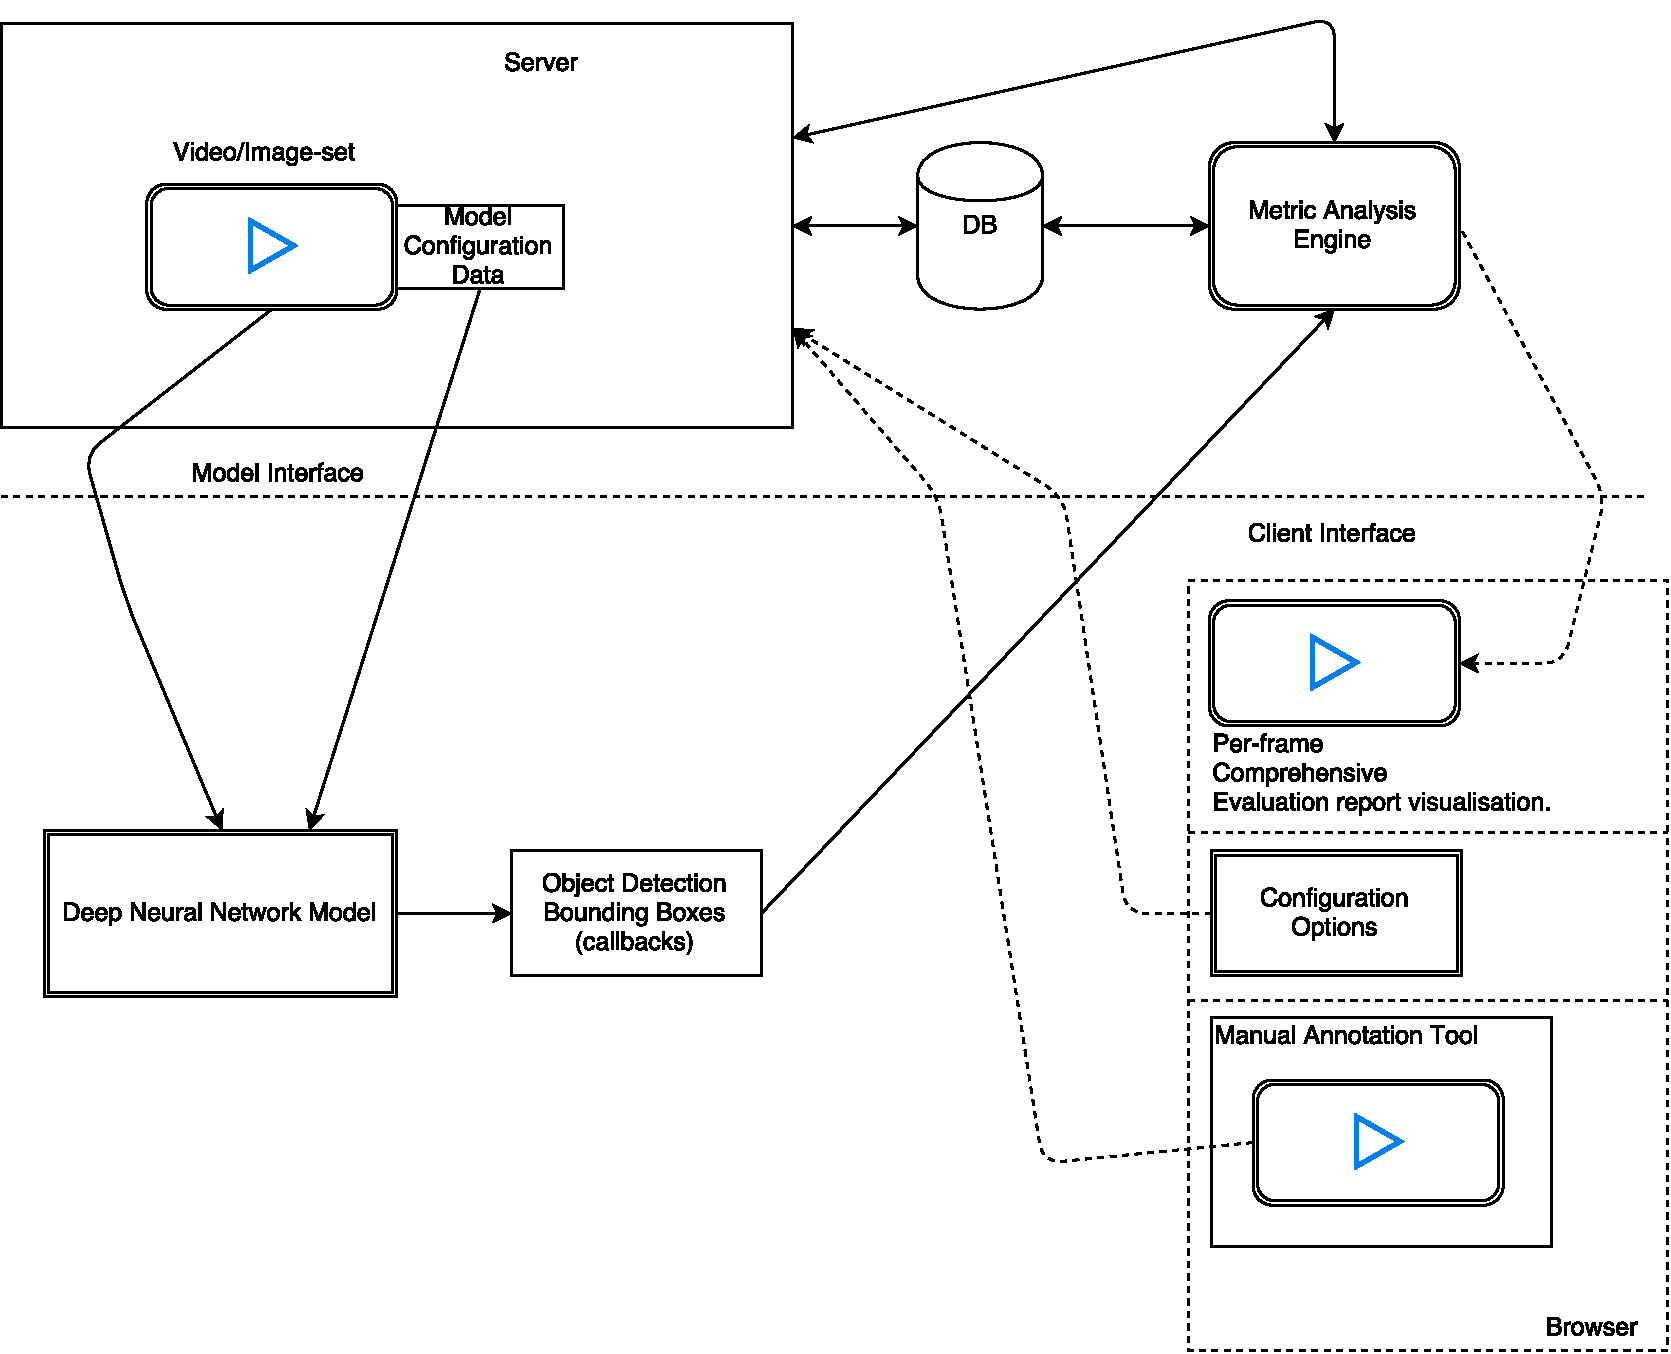
\includegraphics[width=\figwidthb]{fig/system_architecture.pdf}
\caption{System Architecture.} \label{fig.structure}
\end{figure}

\subsubsection{Server}
There shall be a web server hosted with the video/image-set database. The server implements basic video annotation features like user-account, video annotation data and label management. There can be administrator users and staff users. Administrator will be able to add/delete users, add/delete video annotation jobs, add/delete classification labels for annotaion. Staff users will be able to view the video annotation jobs and annotate appropriately the objects identified under the list of provided labels.
\subsubsection{Model interface (MI)}
The model-interface defines an extensive API, bridging the communication between the Server and deep-learning neural network models under research.
\subsubsection{A deep neural network model (DNN)}
A deep learning neural network model like the convolutional (CNN) YOLO model which was used to implement the system discussed in this paper.
\subsubsection{Metric analysis engine (MAE)}
The metric analysis engine appropriately calculate the progress-metric as discussed in the workflow section below.
\subsubsection{Client interface (CI)}
The client interface is managed by the web server.
\subsubsection{Browser}
The client browser shall render the user interfaces for:
\begin{itemize}
	\item Manual video annotation and corrections
	\item DNN model configuration
	\item DNN model run
	\item View comprehensive evaluation
\end{itemize}

\section{Workflow}
\subsection{Data Inference Level}
The tool runs the model with saved configurations on the input video and saves the generated annotation data-set in the database. This enables the researcher to visually see the error and correct any of them. The tool in the background calculates:
\begin{itemize}
	\item the error for each annotation made (at box level).
	\item un-detected objects which the user was able to detect.
	\item And the such.
\end{itemize}

\subsection{Training}
The user can then train the model again with the new data-set. 

\subsection{Loop continues}
The user can now re-iterate the process with another data-inference cycle, pre-processing data and triggering the data-set generation. MAE shall learn the changes with new data-set against the old, backup the accurate manually corrected data and provides the user with the improvement metric and areas at fault. MAE uses video overlays to depict the metric at a frame level over the source video data.

\section{Progress Metric}
The Progress Metric shall be a simple visualization of inference accuracy as detected by MAE. The metric shall consider:
\begin{itemize}
	\item Bounding box precision.
	\item Object prediction accuracy (boolean; whether the object was classified correctly).
	\item Object detection status (boolean; whether the object was detected by the model or was manually labelled after inference).
	\item Object tracking accuracy (if applicable; boolean; whether the object was tracked between adjacent frames).
\end{itemize}
The above evaluated metrics are presented graphically in a table or graph format as shown below. 

\begin{tabular}{| c | c | c | c | c | c | c | }
\hline
Model & Class (CAR)  & & & & Classes \\ 
\hline 
     & tp & tn & fp & fn & AP & mAP \\ 
YOLO & 769 & 0 &  108 & 56 & 0.89 & 0.19  \\
FRCNN & 723 & 0 & 3 & 5 & 0.99 & 0.974 \\
\hline
\end{tabular}


\subsection{Bounding box precision}
<<<<<<< HEAD
We use IoU (Intersection over Union) to measure the bounding box precision. The IoU value is in-turn used to map object bounding boxes between the ground truth and model prediction. 
=======
We use IoU (Intersection over Union) to measure the bounding box precision. The IoU value is in-turn used to map object bounding boxes between the ground truth and model prediction.
>>>>>>> 7b0e570d5ba54e3273ba3b2686855061a0ef154a
\begin{align}
{IoU}={Area of Overlap} / {Area of Union}
\end{align}

%\begin{figure}
%\centering
%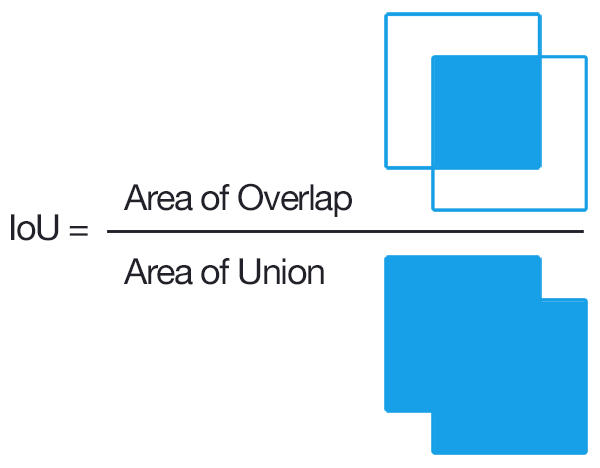
\includegraphics[width=\figwidthb]{fig/iou_equation.png}
%\caption{IoU equation.} \label{fig.structure}
%\end{figure}

\subsection{Accuracy counts}
The accuracy counts calculated for each class/label for the comprehensive evaluation result are:
\begin{itemize}
	\item True Positives (tp). 
	%\begin{displaymath}
	%\mathbf{t}_p
	%\end{displaymath}
	This is the number of bounding boxes classified correctly according to the labels used to train the model. Say, when an object, car is correctly classified as a car.
	\item False Positives (fp).
	%\begin{displaymath}
	%\mathbf{f}_p
	%\end{displaymath}
	This is the number of bounding boxes classified in-correctly according to the labels used to train the model. Say, when an object, car is incorrectly classified as a truck.
	\item True Negatives (tn).
	%\begin{displaymath}
	%\mathbf{t}_n
	%\end{displaymath}
	This is the number of bounding boxes classified correctly as objects the model was not trained for. Say, when an object airplane whose classification is not desired is left unpredicted.
	\item False Negatives (fn).
	%\begin{displaymath}
	%\mathbf{f}_n
	%\end{displaymath}
	This is the number of bounding boxes classified in-correctly as valid objects. Say, when an object airplane whose classification is not desired is classified as a car.
\end{itemize}

\subsection{Precision}
	Precision is the percentage of true positives in the classified objects' list. Thus, precision is a metric associated with a single class.
	\begin{align}
	\mathbf{precision}=\mathbf{t}_p / (\mathbf{t}_p + \mathbf{f}_p) = \mathbf{t}_p / {n}
	\end{align}
	where $\mathbf{n}$ is the total number of objects classified by the model.
\subsection{Recall}
	Recall is the percentage of objects correctly classified. Thus, recall is a metric associated with a single class.
	\begin{align}
	\mathbf{recall}=\mathbf{t}_p / (\mathbf{t}_p + \mathbf{f}_n)
	\end{align}
\subsection{Precision Recall Graph for each class}
	Rule of thumb is that a good model shall maintain high precision and high recall with different threshold values used for the classification score/probability. Thus a precision-recall graph plotted between the precision and recall values of a class across the frame or video for different subsets of predicted output, give us a pretty good visualisation of the model quality. The subset used here is sampled from the list of classified bounding boxes, sorted with the model's score value. The subset shall move from as low as one object to all the objects in the list. Popular evaluation models like the one used with VOC Challenge uses a 11-point sampling, but we propose the more accurate k-point sampling, where we plot precision-recall values for every subset that results a change in the accuracy count metric.
\begin{figure}
\centering
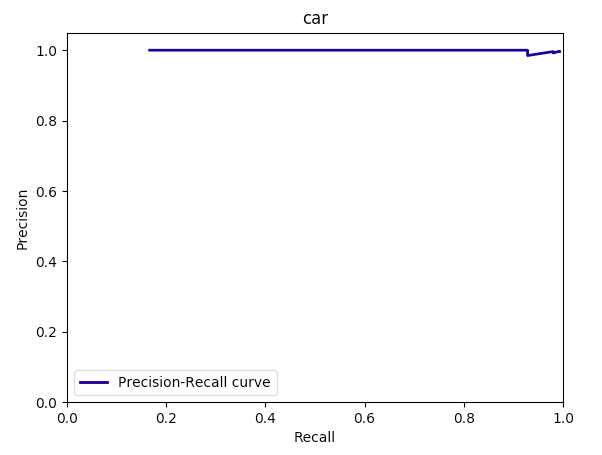
\includegraphics[width=\figwidthb]{fig/pr_rcnn.png}
\caption{Prediction recall curve when we ran RCNN, class "Car" for a 2 second video.} \label{fig.structure}
\end{figure}

\begin{figure}
\centering
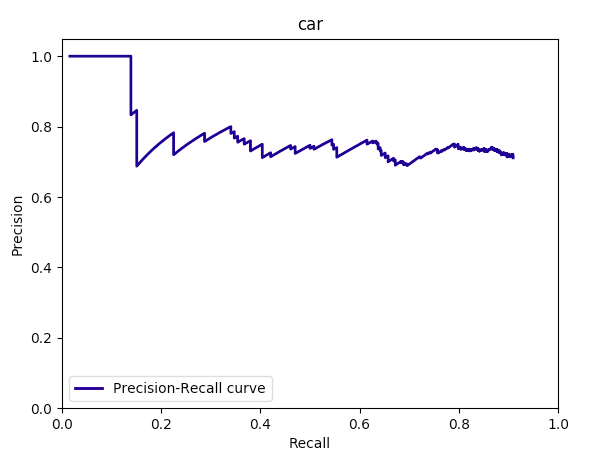
\includegraphics[width=\figwidthb]{fig/pr_yolo.png}
\caption{Prediction recall curve when we ran YOLO, class "Car" for a 2 second video.} \label{fig.structure}
\end{figure}

\subsection{Average Precision for each class}
	Average precision is the single number derived from the above graph, simply by taking the area under the plotted curve.
	$${AP} = \int_{0}^{1} P(r) dr$$
	Practically the area under the curve could be implemented as:
	$${AP} = \sum_{k=1}^{N} P(k) {\Delta}r(k)$$
\subsection{Interpolated Average Precision for each class}
	Interpolated average precision is calculated the same way as we calculated {AP} above, but, instead of using {P(k)}, the maximum precision value: 
	$${max}_{k\textsuperscript{'}>= k} {P(k\textsuperscript{'})}$$
	Thus:
	$${IAP} = \sum_{k=1}^{N} {max}_{k\textsuperscript{'}>= k} {P(k\textsuperscript{'})} {\Delta}r(k)$$

\subsection{Mean Average Precision across all the classes the model was trained on}
	Mean average precision, {mAP} is the mean of the {AP} values calculated for each of the classes supported by the model. 

\subsection{Evaluation User Interface}

	A detailed and comparative visualization of the model output and model result analyses will improve the process of discovering the robustness and vulnerabilities of selected model tremendously. Thus for each model that users selected, the UI of the evaluation panel can be elaborated as follows: \par
	1. Frame by frame video visualization. 
By looking at the ground truth and predicted bounding boxes of one annotated video frame by frame, users can determine the precision of models in an intuitive way.\par
	2. Precision-Recall Curve per frame/video visualization. 
By plotting the Precision-Recall Curve in both specific and conclusive manner, users can review the output of their models from a general but precise angle.\par
	3. True positive, false positive, true negative, false negative and mean Average Precision list visualization. 
With these specific and decisive variables displaying, users can see the correlations between the predicted bounding boxes and ground truth results, as well as the correlations between video bounding box visualization and Precision-Recall Curves.\par
From these perspectives, users now can conceive a comprehensive view of their models, thus improvement and selection for the models can be recognized and achieved easily.


	
%Math symbol: $\hat{r}_{n,m}^{(k)}$.

%Equations:
%\begin{align}
%\mathbf{f}_t^n=\mathbf{R}_b^n \mathbf{f}_t^b + \mathbf{e}^n
%\end{align}
%where $\mathbf{e}^n$ is the error of the force that applied to the smartphone. The figure is shown in \figref{fig.doublefigure} and \figref{fig.structure}.

%\begin{figure}[htb]
%\centerline{\subfloat[Figure 1]{\includegraphics[width
%=0.5\linewidth]{fig/city.pdf} \label{fig.figure1}} \hfil
%\subfloat[Figure 2]{\includegraphics[width=0.5\linewidth]{fig/city.pdf}
%\label{fig.figure2}}
%} \caption{The figure for: (a) Figure1; (b) Figure2.} \label{fig.doublefigure}
%\end{figure}






\section{Related Work}\label{sec.related}

There is a significant amount of image and video data that researchers wish to utilise efficiently. However, without properly label or annotate, the data will become waste. Therefore, developing annotation tools for different purposes is almost as important as these large datasets themselves.

For image annotation, Abhishek Dutta, Ankush Gupta and Andrew Zisserman of the Visual Geometry Group of University of Oxford developed a simple browser-based tool, which supports region shapes of rectangle, circle, ellipse, polygon and point, called VGG Image Annotator (VIA)\cite{abh2017via}, which can be utilised offline with json format output. NVIDIA AI City Challenge 2017 used DMIAT as its annotation platform. Torralba et al(2010)\cite{Russell2008labelme} proposed a LabelMe tool for static image annotation.  

However, the static image annotation tools do not have the capabilities to handle the continuous nature of the video. Consequently there is significant effort in developing annotation tools for video datasets. Ching-Yung et al(2003)\cite{lin2003videoann} developed VideoAnnEx MPEG-7 Annotation Tool. Yuen J, Russell B, Liu C, Torralba A (2009)\cite{yuen2009labelmevideo} introduced LabelMe Video, an open web-based platform can generate event annotations. Carl V, Donald P, Deva R\cite{carl2012vatic} described Video Annotation Tool from Irvine, California (VATIC). Mihalcik D, Doermann D (2003) presented ViPER\cite{mihalcik2003viper}, a local based software for spatial labeling. Anting S\cite{shen2016beaverdam} described BeaverDam, an easy-installed browser-based tool. In order to lower the annotation cost, Ali et al (2011)\cite{ali2011flowboost} present a method that can populate labels and annotations for a video with only few keyframes annotated. BeaverDam and LabelMe Video use linear interpolation. Agarwala et al (2004)\cite{agarwala2004tracker} describe that by using trackers, object tracking between keyframes would be more precise and more appropriate in rotoscoping and animation. I. Kavasidis et al(2012)\cite{I2012GTTool} presented GTTool which uses Snakes\cite{kass1988snakes} (not polygons), Gaussian Mixture Model (GMM)\cite{stauffer1999gmm} and CAMSHIFT\cite{bradski1998camshift} to generate ground truth automatically. Ground Truth Verification Tool (GTVT)\cite{ambardekar2009gtvt} for video surveillance systems uses simple blob tracking\cite{gupte2002sblobtrack} and calculate the accuracy of bounding boxes.

Considering the cost of annotating large volume visual datasets and the limitations of individual worker, tools for annotation is not enough. Ching-Yung et al(2003)\cite{lin2003videoann} proposed the Video Collaboration Annotation Forum as a corporation effort to annotate TRECVID\cite{smeaton2006trecvid} 2003 video set via the VideoAnnEx MPEG-7 Annotation Tool. A. Sorokin and D. Forsyth introduced Amazon Mechanical Turk(AMT)\cite{sorokin2008amt} for labeling vision data. ImageNet\cite{deng2009imgnet} dataset used AMT to clean its candidate images. VATIC and BeaverDam also have AMT interface built in. 

For the Deep Learning purpose, we further developed BeaverDam, combined the evaluation concepts of Pascal VOC challenge\cite{everingham2010vocchallenge}, and created a unique browser-based, user-based, end to end video annotation tool, which integrated with object detection models to reduce the annotation workload.

The need for having an end-to-end pipeline for DNN modelling and training has been tackled by the project named DIGITS. NVIDIA provides DIGITS under the BSD license, available at http://github.com/NVIDIA/DIGITS. The essential difference between DIGITS and the system proposed in this paper is the fact that our system attempts to closely integrate data-set generation techniques like video annotation and modelling together. This substantially mitigate the ordeal involved with training and modelling of deep neural networks.

There are some projects discussing the process of automatically annotating videos using deep learning like \cite{baptist2016automatedendtoend}, with a focus on multimedia archive search-ability. 

\section{Conclusion}\label{sec.conclusion}


% conference papers do not normally have an appendix


% use section* for acknowledgment
%\section*{Acknowledgment}


%The authors would like to thank...





% trigger a \newpage just before the given reference
% number - used to balance the columns on the last page
% adjust value as needed - may need to be readjusted if
% the document is modified later
%\IEEEtriggeratref{8}
% The "triggered" command can be changed if desired:
%\IEEEtriggercmd{\enlargethispage{-5in}}

% references section

% can use a bibliography generated by BibTeX as a .bbl file
% BibTeX documentation can be easily obtained at:
% http://mirror.ctan.org/biblio/bibtex/contrib/doc/
% The IEEEtran BibTeX style support page is at:
% http://www.michaelshell.org/tex/ieeetran/bibtex/
%\bibliographystyle{IEEEtran}
% argument is your BibTeX string definitions and bibliography database(s)
%\bibliography{IEEEabrv,../bib/paper}
%
% <OR> manually copy in the resultant .bbl file
% set second argument of \begin to the number of references
% (used to reserve space for the reference number labels box)

%\bibliographystyle{IEEEtran}
%\bibliography{IEEEmybib}

%\begin{thebibliography}{1}
%
%\bibitem{IEEEhowto:kopka}
%H.~Kopka and P.~W. Daly, \emph{A Guide to \LaTeX}, 3rd~ed.\hskip 1em plus
%  0.5em minus 0.4em\relax Harlow, England: Addison-Wesley, 1999.
%
%\end{thebibliography}

\begin{thebibliography}{9}

\bibitem{baptist2016automatedendtoend} 
B. Vandersmissen et al., "An Automated End-To-End Pipeline for Fine-Grained Video Annotation using Deep Neural Networks," in 
\textit{International Multimedia Conference.}, Amsterdam, 2016, pp.409-412.
 
\bibitem{redmon2016yolo9000} 
J. Redmon and A. Farhadi. (2016, December 25). 
\textit{YOLO9000: Better, Faster, Stronger} (\textit{2nd ed.}) [Online]. Available: https://arxiv.org/abs/1612.08242

\bibitem{vondrick2011vatic}
C. Vondrick et al., "Efficiently Scaling Up Crowdsourced Video Annotation", \textit{International Journal of Computer Vision.}, pp. 0920-5691, June. 2012.

\bibitem{everingham2010vocchallenge}
M. Everingham et al., "The Pascal Visual Object Classes (VOC) Challenge", \textit{International Journal of Computer Vision.}, vol.88, no.2, pp. 303-338, June. 2010.

\bibitem{doennann2000ViPER} 
D. Doennann and D. Mihalcik, "Tools and techniques for video performance evaluation," in 
\textit{Pattern Recognition, 2000. Proceedings. 15th International Conference.}, Barcelona, 2000, pp.167-170. doi: 10.1109/ICPR.2000.902888
    
\bibitem{shen2016beaverdam} 
A. Shen, "BeaverDam: Video Annotation Tool for Computer Vision Training Labels," M.S. thesis, EECS, Univ. California, Berkeley, CA, 2016.

\bibitem{abh2017via}
VGG Image Annotator : Visual Geometry Group. (2017, July 22). Retrieved from http://www.robots.ox.ac.uk/~vgg/software/via/

\bibitem{Russell2008labelme}
B. C. Russell, A. Torralba, K. P. Murphy, and W. T. Freeman, ?Labelme: A database and web-based tool for image annotation,? Int. J. Comput. Vision, vol. 77, no. 1-3, pp. 157?173, May 2008.

\bibitem{lin2003videoann}
C. Lin and B. Tseng, ?Video collaborative annotation forum: Establishing ground-truth labels on large multimedia datasets,? Proceedings of the TRECVID 2003, 2003

\bibitem{yuen2009labelmevideo}
Yuen J, Russell B, Liu C, Torralba A (2009) LabelMe video: Building a Video Database with Human Annotations. International Conference of Computer Vision

\bibitem{carl2012vatic}
Carl Vondrick, Donald Patterson, Deva Ramanan. "Efficiently Scaling Up
Crowdsourced Video Annotation" International Journal of Computer Vision
(IJCV). June 2012.(VATIC)

\bibitem{mihalcik2003viper}
Mihalcik D, Doermann D (2003) The Design and Implementation of ViPER. Technical Report 

\bibitem{ali2011flowboost}
Ali K, Hasler D, Fleuret F (2011) Flowboost? appearance learning from sparsely annotated video. IEEE Computer Vision and Pattern Recognition 

\bibitem{agarwala2004tracker}
Agarwala A, Hertzmann A, Salesin D, Seitz S (2004) Keyframe-based tracking for rotoscoping and animation. In: ACM Transactions on Graphics (TOG), ACM, vol 23, pp 584?591

\bibitem{I2012GTTool}
I. Kavasidis, S. Palazzo, R. Di Salvo, D. Giordano, C. Spampinato (2012), ?A semi-automatic tool for detection and tracking ground truth generation in videos,? Proceedings of the 1st International Workshop on Visual Interfaces for Ground Truth Collection in Computer Vision Applications - VIGTA '12 - 2012

\bibitem{kass1988snakes}
M. Kass, A. Witkin, and D. Terzopoulos, ?Snakes: Active contour models,? International Journal of Computer Vision, vol. 1, no. 4, pp. 321?331, Jan. 1988.	

\bibitem{stauffer1999gmm}
C. Stauffer and W. E. L. Grimson, ?Adaptive background mixture models for real-time tracking,? Computer Vision and Pattern Recognition, IEEE Computer Society Conference on, vol. 2, pp. 246?252, 1999.

\bibitem{bradski1998camshift}
G. R. Bradski, ?Computer Vision Face Tracking For Use in a Perceptual User Interface,? Intel Technology Journal, pp. 1?15, 1998.

\bibitem{ambardekar2009gtvt}
A. Ambardekar and M. Nicolescu, ?Ground Truth Verification Tool (GTVT) for Video Surveillance Systems,? in Advances in Computer-Human Interactions, 2009. ACHI ?09. Second International Conferences on, Cancun, 2009, pp. 354?359.	

\bibitem{gupte2002sblobtrack}
S. Gupte, O. Masoud, R. F. K. Martin, and N. P. Papanikolopoulos, ?Detection and Classification of Vehicles,? IEEE Transactions on Intelligent Transportation Systems, vol. 3, no. 1, pp. 37-47, 2002. 

\bibitem{smeaton2006trecvid}
Smeaton A, Over P, Kraaij W (2006) Evaluation campaigns and trecvid. In: Proceedings of the 8th ACM international workshop on Multimedia information retrieval, ACM, pp 321?330

\bibitem{sorokin2008amt}
A. Sorokin and D. Forsyth. Utility data annotation with amazon mechanical turk. In InterNet08, pages 1?8, 2008.

\bibitem{deng2009imgnet}
J. Deng, W. Dong, R. Socher, L.-J. Li, K. Li, and L. Fei-Fei, ?ImageNet: A Large-Scale Hierarchical Image Database,? in CVPR09, 2009.

\end{thebibliography}
% that's all folks
\end{document}


